\section{Auswertung}

\subsection{Dichtebestimmung}

\begin{itemize}
  \item Masse des runden Stabes: $m_{\text{rund}} = \SI{379,2}{\g}$
  \item Masse des eckigen Stabes: $m_{\text{eckig}} = \SI{167,1}{\g}$
  \item Gesamtlänge des runden Stabes: $L_{\text{ges, rund}} = \SI{57,5}{\cm}$
  \item Gesamtlänge des eckigen Stabes: $L_{\text{ges, eckig}} = \SI{59,0}{\cm}$
  \item Erdbeschleunigung: $g = \SI{10}{\meter \per \square \second}$
  \item Radius des rundes Stabes: $r= \SI {0,5}{cm}$
  \item Seitenlängen a und b des eckigen Stabes: $a=b=\SI{1}{cm}=h$
\end{itemize}

Wie in \ref{sec:dichte} beschrieben, werden nun die Dichten der beide Stäbe berechnet:

\begin{align*}
  \rho_{\text{rund}} &= \SI{8396,74}{\kilo \gram \per \cubic \meter}\\
  \rho_{\text{eckig}} &= \SI{2832,20}{\kilo \gram \per \cubic \meter}
\end{align*}

Laut \cite{dichte} entspricht $\rho_{\text{rund}}$ der Dichte von Messing und $\rho_{\text{eckig}}$ der
Dichte von Aluminium.

\newpage

\subsection{Einseitge Einspannung}

\subsubsection{Runder Stab}

Die eigentliche Auslenkung $D(x)$ berechnet sich aus $D_m(x) - D_0(x)$ und die eingespannte Länge des
Stabes beträgt $L = \SI{50,1}{\cm}$. Die Masse des angehängten Gewichts beträgt $m=\SI{1183,0}{g}$

\begin{table}[H]
  \centering
  \caption{Messdaten}
  \label{tab:rundein}
  \begin{tabular}{S S S S }
    \toprule
      {$x \:/\: \mathrm{cm}$} & {$D_0(x) \:/\: \mathrm{mm}$} & {$D_m(x) \:/\: \mathrm{mm}$} &
      {$D(x) \:/\: \mathrm{mm}$} \\
    \midrule
    3  &  0,00  &  0,15  &  0,15  \\
    5  &  0,01  &  0,21  &  0,20  \\
    7  &  0,03  &  0,38  &  0,35  \\
    9  &  0,08  &  0,61  &  0,53  \\
    11  &  0,14  &  0,92  &  0,78 \\
    13  &  0,16  &  1,18  &  1,02 \\
    15  &  0,27  &  1,59  &  1,32 \\
    17  &  0,42  &  2,07  &  1,65 \\
    19  &  0,41  &  2,62  &  2,21 \\
    21  &  0,54  &  2,94  &  2,40 \\
    23  &  0,61  &  3,45  &  2,84 \\
    25  &  0,76  &  4,05  &  3,29 \\
    27  &  0,91  &  4,77  &  3,86 \\
    29  &  1,09  &  5,33  &  4,24 \\
    31  &  1,26  &  6,00  &  4,74 \\
    33  &  1,36  &  7,01  &  5,65 \\
    35  &  1,59  &  7,54  &  5,95 \\
    37  &  1,87  &  8,25  &  6,38 \\
    39  &  2,05  &  9,06  &  7,01 \\
    41  &  2,24  &  9,79  &  7,55 \\
    \bottomrule
  \end{tabular}
\end{table}

\newpage

Aus diesen Messwerten folgt der Graph:

\begin{figure}[H]
  \centering
  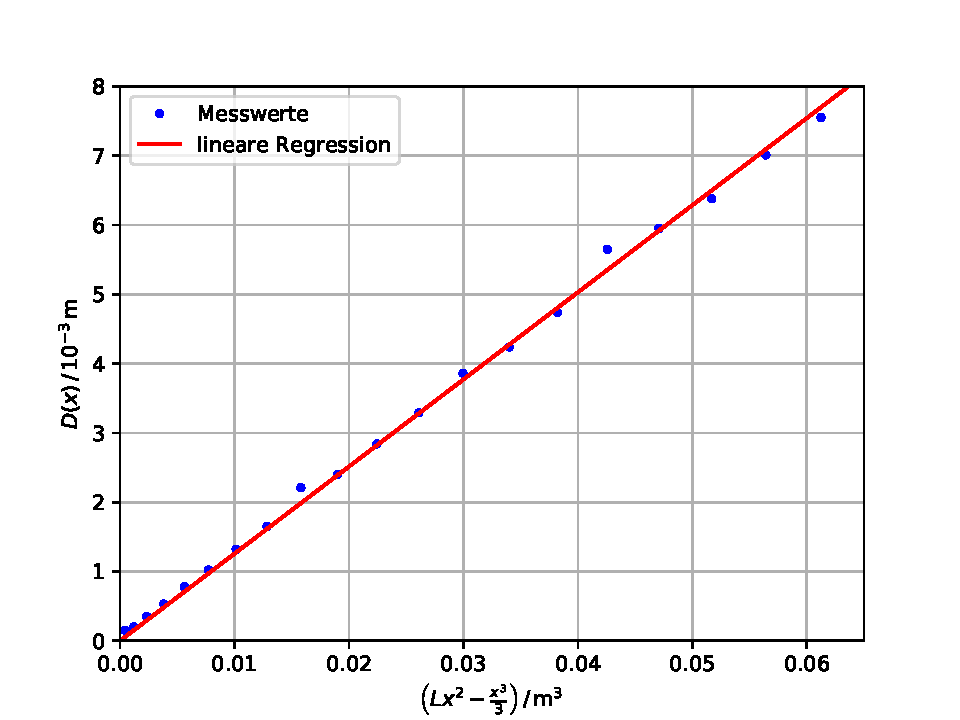
\includegraphics[width=\textwidth]{Plots/rundein.pdf}
  \caption{$\left(L x^2 - \frac{x^3}{3}\right)$-$D(x)$-Diagramm zur Bestimmung des Elastizitätsmoduls}
  \label{fig:rundein}
\end{figure}

Zur Bestimmung des Elastizitätsmoduls wird eine lineare Regression durchgeführt, die folgende Werte liefert:

\begin{table}[H]
  \centering
  \caption{lineare Regression}
  \label{tab:lin1}
  \begin{tabular}{l c}
    \toprule
       & {Werte}\\
    \midrule
    Steigung m & \SI{0.1257(8)}{1 \per \square \meter} \\
    %Achsenabschnitt b & \SI{9.0035(3446)e-5}{\meter} \\
    \bottomrule
  \end{tabular}
\end{table}


Der Elastizitätsmodul $E = \SI{95,86(60)}{\giga \pascal}$
ergibt sich aus Gleichung \eqref{eqn:ein}.
Das benötigte Flächenträgheitsmoment eines Kreisquerschnittes \cite{traeg} ist

\begin{equation}
  I_{\text{Kreis}} = \frac{\pi r^4}{4}.
\end{equation}

Den Fehler erhält man aus der Gauß'schen Fehlerfortpflanzung

\begin{equation}
   \delta = \sqrt{ \sum_{i=1}^{n}(\frac{\partial y}{\partial x_i} \Delta x_i)^2}.
   \label{eqn:gaus}
 \end{equation}

\subsubsection{Eckiger Stab}

Wie schon im vorausgegangenen Kapitel berechnet sich auch hier
die benötigte Auslenkung als $D(x) = D_m(x) - D_0(x)$.
Dieses mal ist die eingespannte Stablänge $L = \SI{49,9}{\cm}$ und das eingespannte Gewicht beträgt $m=\SI{1202,1}{g}$
Alle benötigten Messdaten finden sich in nachfolgender Tabelle:

\begin{table}[H]
  \centering
  \caption{Messdaten}
  \label{tab:eckigein}
  \begin{tabular}{S S S S }
    \toprule
      {$x \:/\: \mathrm{cm}$} & {$D_0(x) \:/\: \mathrm{mm}$} & {$D_m(x) \:/\: \mathrm{mm}$} &
      {$D(x) \:/\: \mathrm{mm}$} \\
    \midrule
    3  &  0,00  &  0,09  &  0,09   \\
    5  &  0,00  &  0,18  &  0,18   \\
    7  &  0,03  &  0,34  &  0,31   \\
    9  &  0,12  &  0,58  &  0,46   \\
    11  &  0,25  &  0,95  &  0,70  \\
    13  &  0,45  &  1,35  &  0,90  \\
    15  &  0,66  &  1,80  &  1,14  \\
    17  &  0,88  &  2,30  &  1,42  \\
    19  &  1,13  &  2,93  &  1,80  \\
    21  &  1,42  &  3,48  &  2,06  \\
    23  &  1,65  &  4,11  &  2,46  \\
    25  &  1,93  &  4,75  &  2,82  \\
    27  &  2,21  &  5,41  &  3,20  \\
    29  &  2,46  &  6,12  &  3,66  \\
    31  &  2,75  &  6,82  &  4,07  \\
    33  &  3,06  &  7,53  &  4,47  \\
    35  &  3,30  &  8,23  &  4,93  \\
    37  &  3,55  &  8,93  &  5,38  \\
    39  &  3,85  &  9,65  &  5,80  \\
    \bottomrule
  \end{tabular}
\end{table}

\newpage

Daraus folgt der Graph:

\begin{figure}[H]
  \centering
  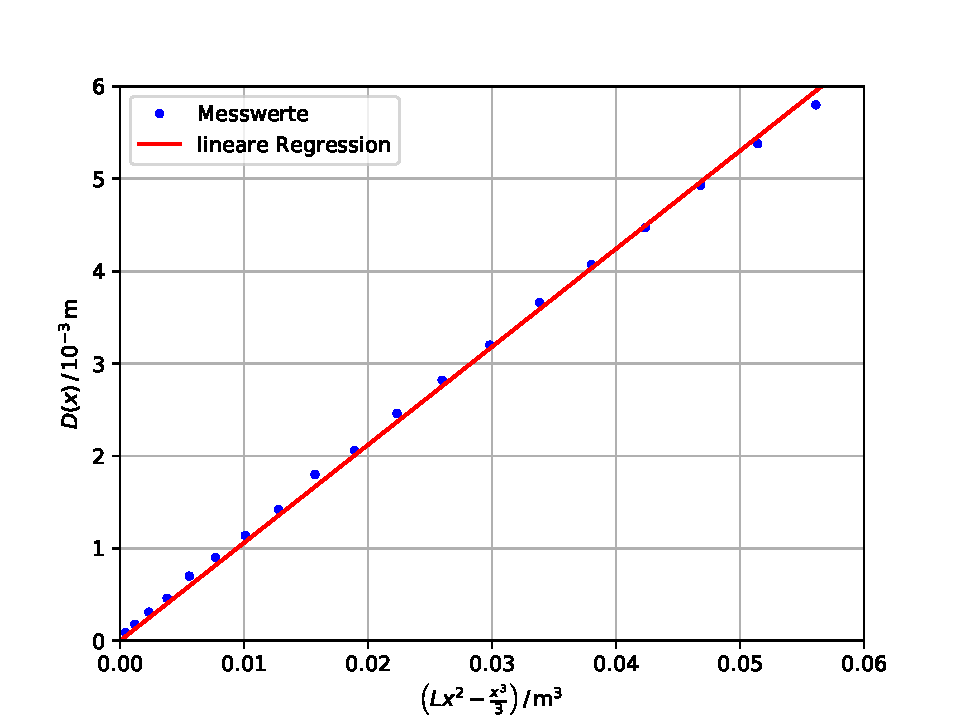
\includegraphics[width=\textwidth]{Plots/eckigein.pdf}
  \caption{$\left(L x^2 - \frac{x^3}{3}\right)$-$D(x)$-Diagramm zur Bestimmung des Elastizitätsmoduls}
  \label{fig:eckigein}
\end{figure}

\begin{table}[H]
  \centering
  \caption{lineare Regression}
  \label{tab:lin2}
  \begin{tabular}{l c}
    \toprule
       & {Werte}\\
    \midrule
    Steigung m & \SI{0.1060(4)}{1 \per \square \meter} \\
    %Achsenabschnitt b & \SI{0.0001(0)}{\meter} \\
    \bottomrule
  \end{tabular}
\end{table}

Aus Gleichung \eqref{eqn:ein} berechnet sich der Elastizitätsmodul mit dem Fehler aus Gleichung \eqref{eqn:gaus}
$E = \SI{68,01(40)}{\giga \pascal}$.
Das Flächenträgheitsmoment einer quadratischen Querschnittsfläche \cite{traeg} ist

\begin{equation}
  T_{\text{Quadrat}} = \frac{h^4}{12}.
\end{equation}
%\newpage

\subsection{Beidseitige Einspannung - Runder Stab}

Die eingespannte Länge zwischen den beiden Punkten A und B (s. \ref{fig:Aufbau}) beträgt $L = \SI{54,5(0)}{\cm}$.
Das Gewicht hat hier eine Masse von $m=\SI{3541,3}{g}$.
Für die Messung wurde Punkt A als Startpunkt, also $x = 0$, ausgewählt.
Die erste Tabelle zeigt die Messwerte für $0 \leq x \leq \sfrac{L}{2}$
und die zweite Tabelle die Messwerte für $\sfrac{L}{2} \leq x \leq L$.

\begin{table}[H]
  \centering
  \caption{Messdaten - erste Hälfte}
  \label{tab:rundbeid1}
  \begin{tabular}{S S S S}
    \toprule
      {$x \:/\: \mathrm{cm}$} & {$D_0(x) \:/\: \mathrm{mm}$} & {$D_m(x)  \:/\: \mathrm{mm}$} &
      {$D(x) \:/\: \mathrm{mm}$}\\
    \midrule
    3  &  0,00  &  0,07  &  0,07    \\
    5  &  -0,01  &  0,12  &  0,13   \\
    7  &  -0,02  &  0,18  &  0,20   \\
    9  &  -0,07  &  0,24  &  0,31   \\
    11  &  -0,08  &  0,36  &  0,44  \\
    13  &  -0,03  &  0,49  &  0,52  \\
    15  &  -0,03  &  0,61  &  0,64  \\
    17  &  -0,01  &  0,75  &  0,76  \\
    19  &  0,02  &  0,89  &  0,87   \\
    21  &  0,01  &  0,99  &  0,98   \\
    23  &  0,07  &  1,11  &  1,04   \\
    25  &  0,09  &  1,21  &  1,12   \\
    27  &  0,12  &  1,30  &  1,18   \\
    \bottomrule
  \end{tabular}
\end{table}

\begin{table}[H]
  \centering
  \caption{Messdaten - zweite Hälfte}
  \label{tab:rundbeid2}
  \begin{tabular}{S S S S}
    \toprule
      {$x \:/\: \mathrm{cm}$} & {$D_0(x) \:/\: \mathrm{mm}$} & {$D_m(x)  \:/\: \mathrm{mm}$} &
      {$D(x) \:/\: \mathrm{mm}$}\\
    \midrule
    29,50  &  -0,87  &  0,35  &  1,22  \\
    31,50  &  -0,80  &  0,38  &  1,18  \\
    33,50  &  -0,78  &  0,39  &  1,17  \\
    35,50  &  -0,73  &  0,39  &  1,12  \\
    37,50  &  -0,60  &  0,42  &  1,02  \\
    39,50  &  -0,54  &  0,43  &  0,97  \\
    41,50  &  -0,43  &  0,44  &  0,87  \\
    43,50  &  -0,33  &  0,43  &  0,76  \\
    45,50  &  -0,23  &  0,42  &  0,65  \\
    47,50  &  -0,12  &  0,39  &  0,51  \\
    49,50  &  -0,05  &  0,35  &  0,40  \\
    51,50  &  0,00  &  0,24  &  0,24  \\
    \bottomrule
  \end{tabular}
\end{table}

% Die Fehler von $T_{\diameter}$, die der Formel
%
% \begin{equation}
%   \delta = \sqrt{\frac{1}{n^2-n} \cdot \sum_{i=1}^{n}(x_i - \bar {x})^2}
% \end{equation}
%
% entstammen, ergeben in Kombination mit der Gauß'schen Fehlerfortpflanzung
%
% \begin{equation}
%   \delta = \sqrt{ \sum_{i=1}^{n}(\frac{\partial y}{\partial x_i} \Delta x_i)^2}.
% \end{equation}
%
% die Fehler von $\frac {1}{T_{\diameter}}$.
%
\newpage

Die dazugehörigen Graphen sind:

\begin{figure}[H]
  \centering
  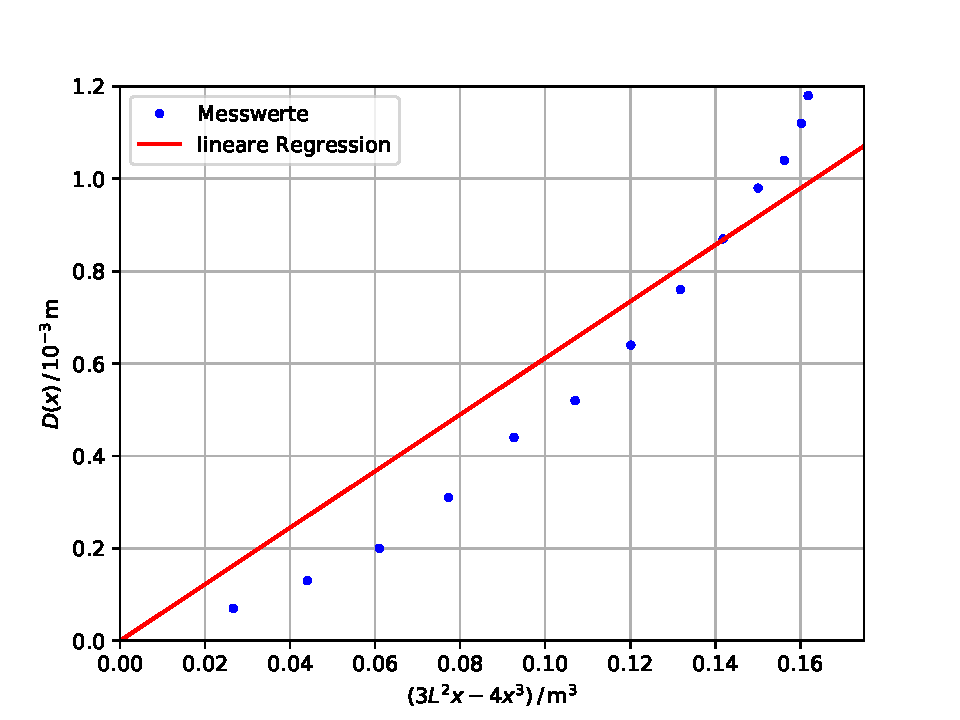
\includegraphics[width=\textwidth]{Plots/rundbeid1.pdf}
  \caption{$D(x)$-$\left(3 L^2 x - 4 x^3\right)$-Diagramm zur Bestimmung des Elastizitätsmoduls}
  \label{fig:rundbeid1}
\end{figure}

\begin{figure}[H]
  \centering
  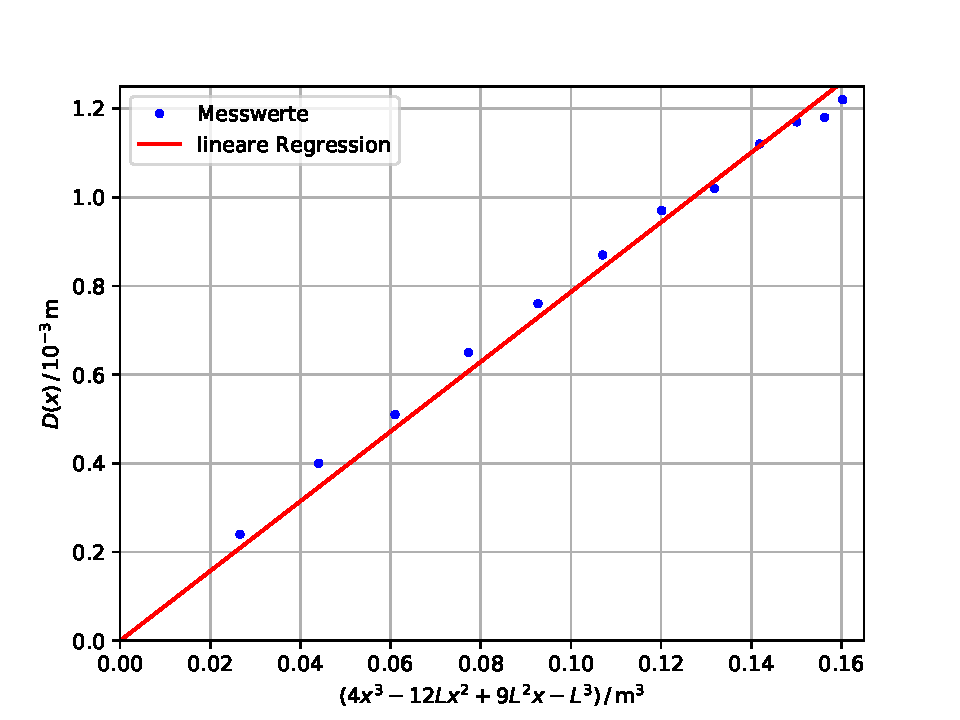
\includegraphics[width=\textwidth]{Plots/rundbeid2.pdf}
  \caption{$D(x)$-$\left(4 x^3 - 12 L x^2 + 9  L^2  x - L^3\right)$-Diagramm zur Bestimmung des Elastizitätsmoduls}
  \label{fig:rundbeid2}
\end{figure}

Hier ergibt sich aus der linearen Regression von Abbildung \ref{fig:rundbeid1}

\begin{table}[H]
  \centering
  \caption{lineare Regression 1}
  \label{tab:lin3}
  \begin{tabular}{l c}
    \toprule
       & {Werte}\\
    \midrule
    Steigung m & \SI{0,0061(3)}{1 \per \square \meter} \\
    %Achsenabschnitt b & \SI{-0,0003(0)}{\meter} \\
    \bottomrule
  \end{tabular}
\end{table}

und den Gleichungen \eqref{eqn:beid1} und \eqref{eqn:gaus}
der Elastizitätsmodul $E_1 = \SI{245,63(1200)}{\giga \pascal}$.

Aus der linearen Regression von Abbildung \ref{fig:rundbeid2}

\begin{table}[H]
  \centering
  \caption{lineare Regression 2}
  \label{tab:lin4}
  \begin{tabular}{l c}
    \toprule
       & {Werte}\\
    \midrule
    Steigung m & \SI{0,0078(9)}{1 \per \square \meter} \\
    %Achsenabschnitt b & \SI{7,4501(14545)}{\meter} \\
    \bottomrule
  \end{tabular}
\end{table}

und Gleichung \eqref{eqn:beid2} ergibt sich mit dem Gauß-Fehler \eqref{eqn:gaus}
der Elastizitätsmodul $E_2 = \SI{191,13(214)}{\giga \pascal}$.

Aus dem Mittelwert von $E_1$ und $E_2$ und dem Fehler aus Gleichung \eqref{eqn:gaus} ergibt sich
$E = \SI{218,38(609)}{\giga \pascal}$.
